\documentclass[twocolumn]{myarticle}

\usepackage{mymacros}
\usepackage{parskip}
\usepackage{hyperref}
\usepackage{listings}
\usepackage{booktabs}

\lstset{%
basicstyle=\small\ttfamily,
columns=flexible,
breaklines=true,
numbers=left,
stepnumber=1,}

\newcommand{\mat}[1]{\begin{bmatrix}#1\end{bmatrix}}
\renewcommand{\d}{\mathrm{d}}

\begin{document}

\title{Physics 581, Assignment 1:\\Monte Carlo methods in computational physics}
\author{Casey Daniel and Chris Deimert}
\date{\today}

\maketitle

\section{Introduction}
\label{sec:introduction}

In this report, we explore a number of Monte Carlo numerical methods.
Monte Carlo methods use pseudorandom numbers to explore complicated systems.
These methods tend to converge slowly for simple problems, but can be very efficient for complex problems: especially those with a large number of variables.

\section{Random number generators}
\label{sec:random_number_generators}

First, we explore the generation of pseudo-random sequences of numbers.
These are key in any Monte Carlo method.

Most often, random number generators try to generate samples of a uniform random variable $ U $, whose probability distribution function is
\begin{align}
    f_U(u) &= \begin{cases} 1 & \text{if } 0 \leq u < 1 \\ 0 & \text{otherwise} \end{cases}
\end{align}
The mean of $ U $ is
\begin{align}
    \mu &= \int_{0}^{1} u \, \d u = \frac{1}{2}.
\end{align}
The variance is
\begin{align}
    \sigma^2 &= \int_0^1 \left(u - \mu\right)^2 \, \d u = \int_{-1/2}^{1/2} u'^2 \, \d u' = \frac{1}{12},
\end{align}
giving standard deviation of
\begin{align}
    \sigma &= \frac{1}{\sqrt{12}}.
\end{align}




%\begin{figure}[ht!]
%    \begin{center}
%    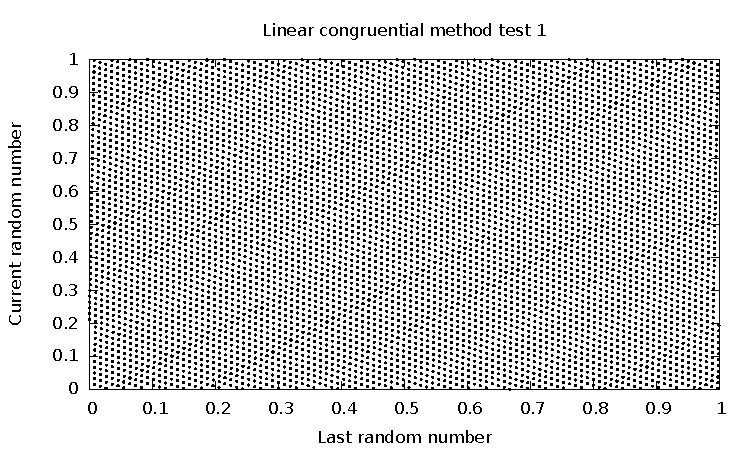
\includegraphics[width = 0.45\textwidth]{../Plots/LCM_test_1.pdf}
%    \caption{%
%        The correlation plot for $ A = 106 $, $ C = 1283 $, and $ M = 6075 $.
%        It is seen that the correlation plot is strongly patterned, meaning that this is a relatively predictable sequence of numbers.
%        Thus, this choice of LCM coefficients is a poor one.
%    }
%    \label{fig:lcm_test_1}
%    \end{center}
%\end{figure}

%\bigskip
%\begin{center}
%    \begin{tabular}{ccccc}
%        \toprule
%        Interval & Upper limit & LCM & gfortran & Exp. \\
%        \midrule
%        1  & 0.1 &  6 &  6 & 10 \\
%        2  & 0.2 & 11 & 16 & 10 \\
%        3  & 0.3 & 12 &  9 & 10 \\
%        4  & 0.4 &  9 &  6 & 10 \\
%        5  & 0.5 & 10 & 11 & 10 \\
%        6  & 0.6 &  9 &  5 & 10 \\
%        7  & 0.7 &  8 & 12 & 10 \\
%        8  & 0.8 & 10 &  9 & 10 \\
%        9  & 0.9 & 11 & 13 & 10 \\
%        10 & 1.0 & 14 & 13 & 10 \\
%        \bottomrule
%    \end{tabular}
%\end{center}
%\bigskip

\onecolumn

\section{Code}
\label{sec:code}

%\lstinputlisting[breaklines]{../../Presentation/Something.f90}
%\vspace{10pt}

\end{document}
